\documentclass{article}
\usepackage[utf8]{inputenc} % UTF-8
\usepackage{amsmath}
\usepackage{amssymb}
\usepackage{algpseudocode} % Algoritmos
\usepackage[a4paper, total={6in, 8in}]{geometry}
\usepackage{graphicx} % Figuras e imagenes
\usepackage{multirow} % Combinacion de celdas en tablas
\usepackage{algorithmicx}
\usepackage{fancyhdr} % Cabeceras y pies de pagina
\usepackage[export]{adjustbox} % Subfiguras
\usepackage{subcaption}
\graphicspath{ {images/} } % Ruta a las imagenes

\title{Práctica 2 - Complejidad de $\mathcal{H}$ y modelos lineales}
\author{Luis Miguel Guirado Bautista - Universidad de Granada}
\date{1 de Mayo de 2022}

\pagestyle{fancy}
\fancyhf{}

% do-while en algoritmos
\algdef{SE}[DOWHILE]{Do}{doWhile}{\algorithmicdo}[1]{\algorithmicwhile\ #1}%

\renewcommand*\contentsname{Índice} % Nombre del indice
\renewcommand{\figurename}{Figura} % Nombre de una figura
\renewcommand{\partname}{Ejercicio} % Nombre de \part
\renewcommand{\familydefault}{\sfdefault}

\begin{document}

    \begin{titlepage}
        \maketitle
        \thispagestyle{empty}
    \end{titlepage}

    \pagebreak

    \lhead{Práctica 2 - Complejidad de $\mathcal{H}$ y modelos lineales}
    \rhead{Luis Miguel Guirado Bautista}
    \tableofcontents

    \pagebreak
    \rfoot{\thepage}
    \section{Complejidad de $\mathcal{H}$ y el ruido}

    \paragraph*{Nota}Para la obtención de resultados se ha ajustado la semilla
    de \texttt{NumPy} a 1

    \subsection*{Funciones usadas}

    \begin{enumerate}
        \item[-]\texttt{simula\_unif(N, dim, rango)} \par 
        Genera \texttt{N} vectores aleatorios uniformes de dimensión \texttt{dim}.
        dentro del \texttt{rango}

        \begin{figure*}[h]
            \centering
            \caption{Datos generados por \texttt{simula\_unif(N=50, dim=2, rango=[-50,50])}}
            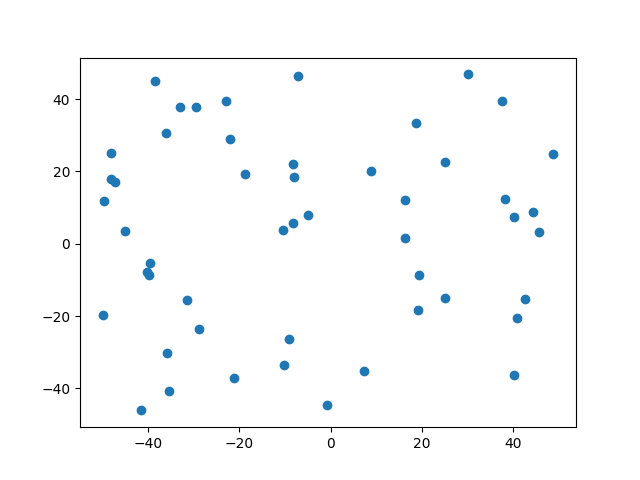
\includegraphics[width=0.7\textwidth]{uniform.png}
        \end{figure*}
        \pagebreak
        \item[-]\texttt{simula\_gauss(N, dim, sigma)} \par
        Genera \texttt{N} vectores aleatorios  de dimensión \texttt{dim} dentro de una distribución Gaussiana.

        \texttt{sigma} es un vector de dimensión \texttt{dim} que posee el valor de la varianza en la
        distribución Gaussiana para cada una de las dimensiones.
        \begin{figure*}[h]
            \centering
            \caption{Datos generados por \texttt{simula\_gauss(N=50, dim=2, sigma=[5,7])}}
            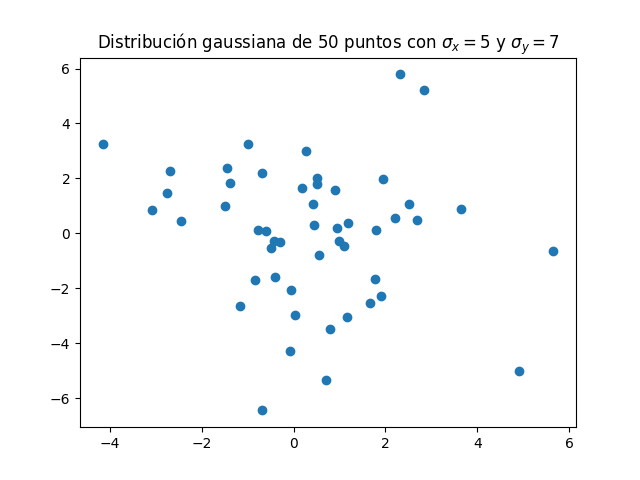
\includegraphics[width=0.7\textwidth]{gauss.png}
        \end{figure*}
        \pagebreak
        \item[-]\texttt{simula\_recta(intervalo)} \par
        Simula una recta del tipo $y = ax + b$ aleatoria con valores dentro de \texttt{intervalo}.

        Devuelve los coeficientes $a$ y $b$.
        \begin{figure*}[h]
            \centering
            \caption{Recta generada por \texttt{simula\_recta(intervalo=[-50,50])}}
            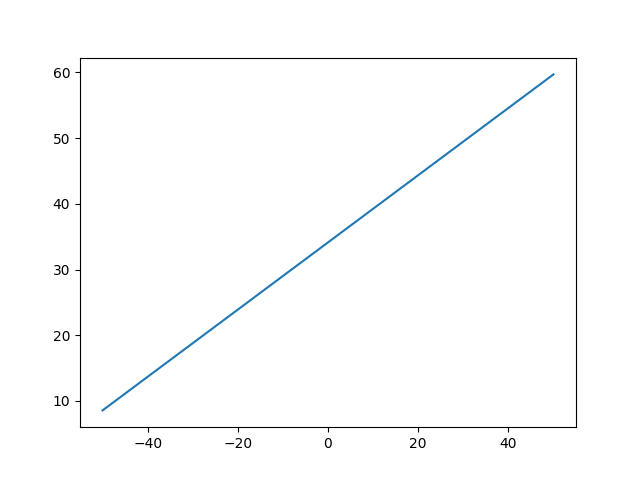
\includegraphics[width=0.7\textwidth]{recta.png}
        \end{figure*}
    \end{enumerate}
    \pagebreak

    \subsection{Influencia del ruido en la selección de la complejidad de $\mathcal{H}$}

    Vamos a generar una muestra aleatoria uniforme con \texttt{simula\_unif(100, 2, [-50,50])}, y vamos a
    clasificar los puntos según la siguiente función:

    \begin{equation*}
        f(x, y) = sign(y - ax - b)
    \end{equation*}

    Donde la tupla $(x,y)$ representa las coordenadas del punto de la función y la tupla $(a,b)$
    representa los coeficientes de la recta $r = ax + b$, generados por la función \texttt{simula\_recta}.
    
    Los coeficientes generados son $a = -0.677$ y $b = -18.89$, de modo que $f$ pasa a ser:

    \begin{equation*}
        f(x, y) = sign(y + 0.667x + 18.89)
    \end{equation*}

    Y la recta que clasifica los puntos es:

    \begin{equation*}
        r = -0.677x - 18.89
    \end{equation*}

    \begin{figure}[h]
        \centering
        %\caption{Grafico con los puntos generados y la recta que los clasifica}
        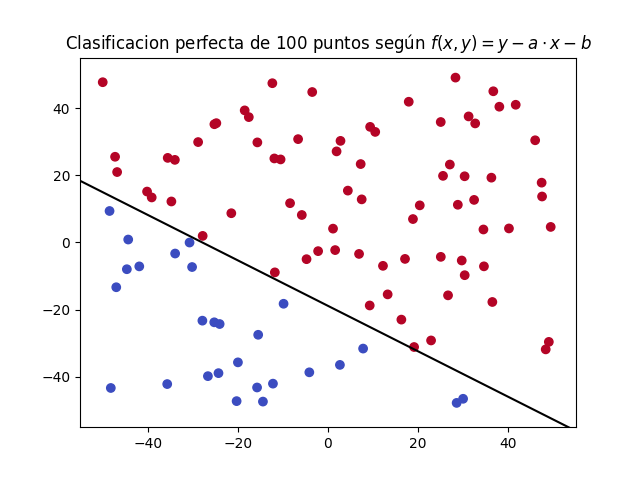
\includegraphics[width=0.7\textwidth]{perfecto.png}
    \end{figure}

    Donde los puntos rojos tienen etiqueta positiva (+1) y los puntos azules
    tienen etiqueta negativa (-1)

    \begin{figure*}[h]
        \centering
        \begin{tabular}{ |c|c| }
            \hline
            $f$ & Proporción(\%) \\
            \hline
            $+1$              & 73  \\
            \hline
            $-1$              & 27 \\
            \hline
        \end{tabular}
    \end{figure*}
    Como la clasificación es perfecta, $E_{in} = 0$.

    \pagebreak

    Ahora vamos a cambiar la clasificación del 10\% de los puntos etiquetados positivamente y otro 10\%
    de los puntos clasificados negativamente.

    \begin{figure}[h]
        \centering
        %\caption{Clasificacion anterior con un 10\% de ruido en ambos subconjuntos}
        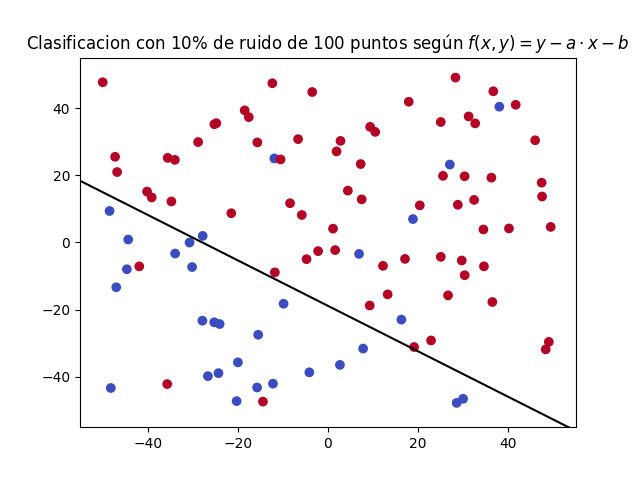
\includegraphics[width=0.7\textwidth]{ruido.png}
    \end{figure}

    \begin{figure*}[h]
        \centering
        \begin{tabular}{ |c|c|c| }
            \hline
            $f$ & Proporción(\%) & Puntos de ruido\\
            \hline
            $+1$              & 69 & 7 \\
            \hline
            $-1$              & 31 & 3 \\
            \hline
        \end{tabular}
    \end{figure*}

    Como 10 puntos de 100 están mal clasificados, entonces

    \begin{equation*}
        E_{in} = \frac{10}{100} = 0.1
    \end{equation*}

    \pagebreak

    Ahora si decidimos cambiar la frontera de clasificación por estas funciones no lineales

    \begin{figure}[h]
        \centering
        \begin{tabular}{ ll }
            $f_1(x,y) = (x - 10)^2 + (y - 20)^2 - 400$ & $f_2(x,y) = 0.5(x+10)^2 + (y-20)^2 - 400$ \\
            $f_3(x,y) = 0.5(x+10)^2 - (y+20)^2 - 400$ & $f_4(x,y) = y - 20x^2 - 5x + 3$ \\
        \end{tabular}
    \end{figure}

    \begin{figure}[h]
        \centering
        %\caption{Clasificacion perfecta de la muestra con 4 funciones no lineales}
        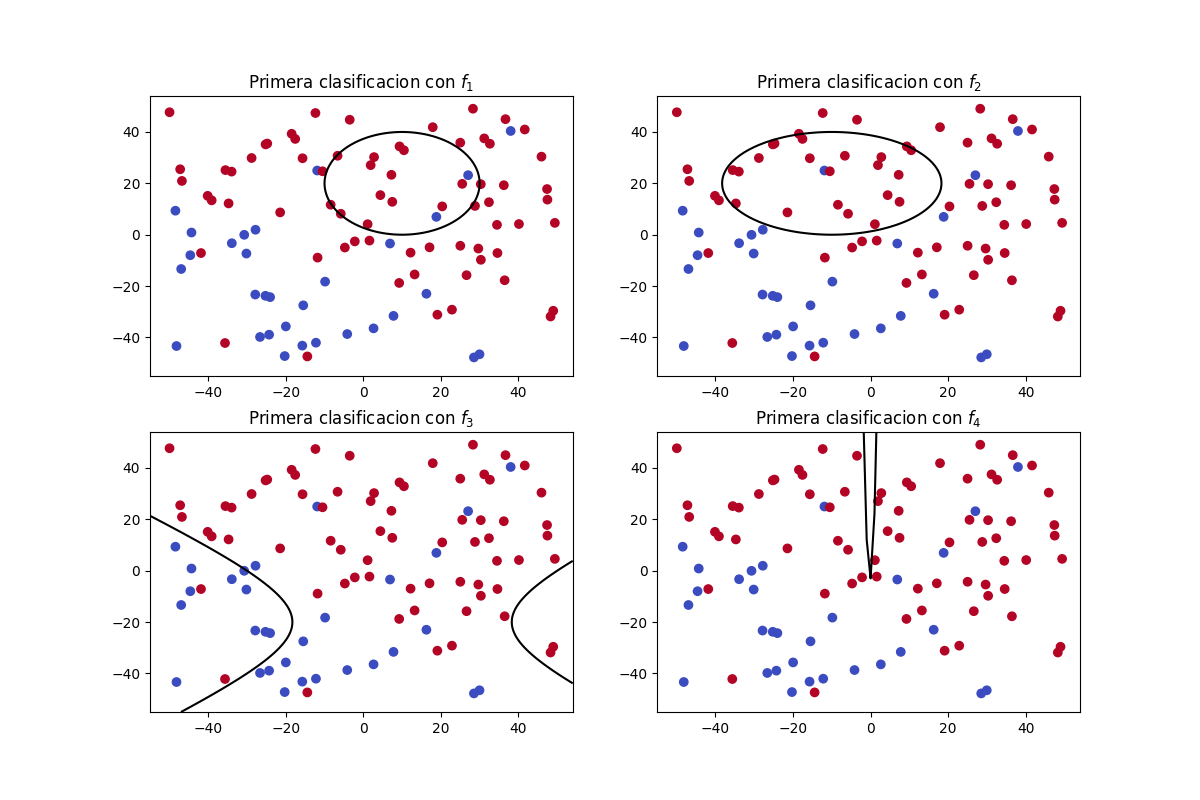
\includegraphics[width=0.9\textwidth]{fall.png}
    \end{figure}

    Obtenemos los siguientes errores de clasificación:

    \begin{figure}[h]
    \centering
    \begin{tabular}{ |c|c|c| }
        \hline
        $f$   & $E_{in}$   \\
        \hline
        $f_1$ & 0.41       \\
        \hline
        $f_2$ & 0.51       \\
        \hline
        $f_3$ & 0.76       \\
        \hline
        $f_4$ & 0.69       \\
        \hline
    \end{tabular}
    \end{figure}

    Podemos observar que $f_3$ es el que peor clasifica los puntos con respecto a $f$, mientras
    el que mejor lo hace es $f_1$.

    Aclaramos que las etiquetas son las mismas que en
    la página anterior, por tanto, la tabla de la página anterior también es aplicable.

    \pagebreak

    Si ahora generamos etiquetas con un 10\% de ruido para cada una de las fronteras:

    \begin{figure}[h]
        \centering
        %\caption{Clasificacion con ruido de la muestra con 4 funciones no lineales}
        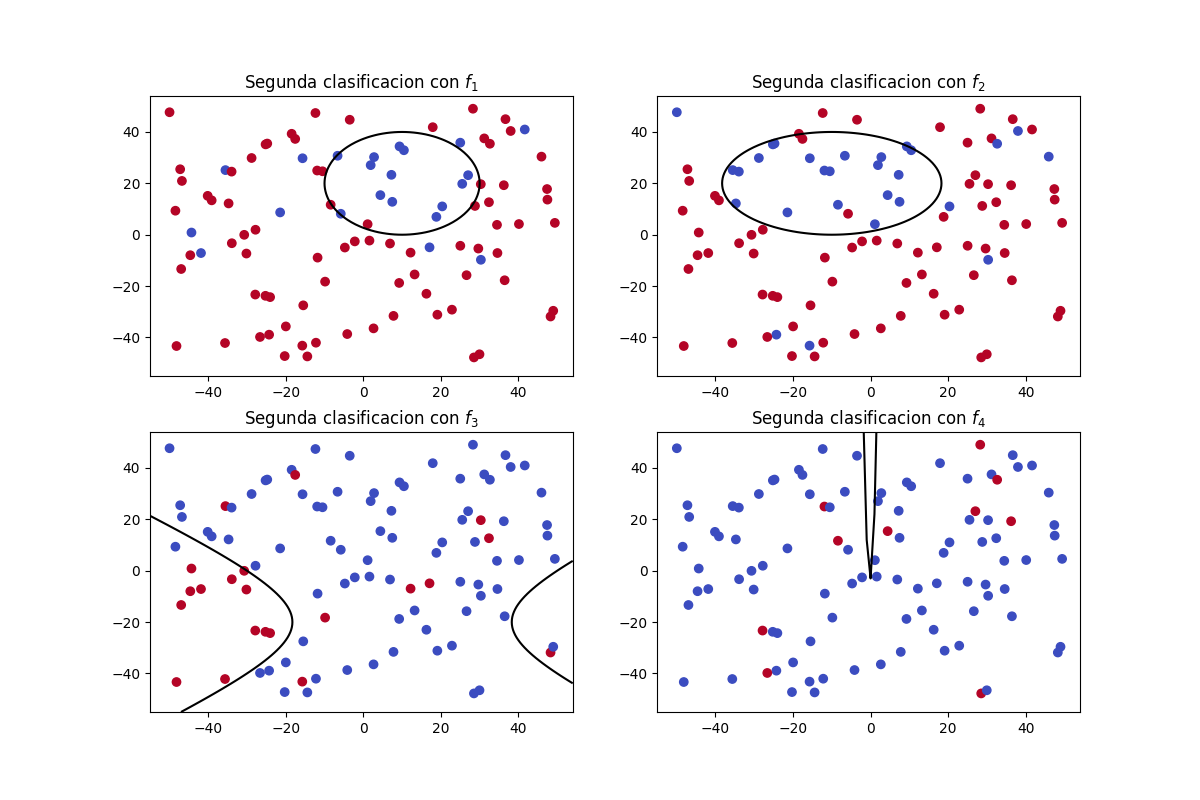
\includegraphics[width=0.9\textwidth]{fallruido.png}
    \end{figure}

    \begin{figure}[h]
    \centering
    \begin{tabular}{ |c|c|c|c| }
        \hline
        $f$                    & Etiqueta & Proporción(\%) & Puntos de ruido \\
        \hline
        \multirow{2}{*}{$f_1$} & +1       & 78             & 9               \\
                               & -1       & 22             & 1               \\
        \hline
        \multirow{2}{*}{$f_2$} & +1       & 72             & 8               \\
                               & -1       & 28             & 2               \\
        \hline
        \multirow{2}{*}{$f_3$} & +1       & 21             & 2               \\
                               & -1       & 79             & 8               \\
        \hline
        \multirow{2}{*}{$f_4$} & +1       & 10             & 0               \\
                               & -1       & 90             & 10              \\
        \hline
    \end{tabular}
    \end{figure}

    Como hemos aplicado un 10\% de ruido a clasificaciones perfectas: $E_{in} = $ 0.1

    \pagebreak

    \section*{Conclusiones}

    Podemos observar en la página 7 que los errores obtendidos con los clasificadores
    no lineales $\{f_1, f_2, f_3, f_4\}$ es mayor que el error del clasificador lineal
    con ruido en la página 6 ($0.1$)
    Por tanto, podemos decir que
    \textbf{no existe correlación directa entre el nivel de complejidad del modelo y la "figura"
    que forman las etiquetas en el plano}, es decir,
    fronteras de clasificación más complejas no tienen
    por que clasificar los resultados mejor, como hemos podido observar en los gráficos anteriores.
    
    También podemos observar que el error de clasificación en $f_4$ en la página 7 se corresponde con
    la proporción de etiquetas $+1$. Es decir, todos los puntos con esta etiqueta
    están mal clasificados porque se encuentran en la región de etiquetas $-1$. Esto se debe
    a que la región $+1$ es demasiado pequeña y por tanto, ningún punto se encuentra dentro de ella.

    Si generamos ruido respecto a $f$ después de clasificar los puntos según $f$, es imposible que
    $E_{in} < 0.1$ o análogamente, \textbf{siempre se cumple que} $E_{in} \ge 0.1$
    al realizar clasificación con un 10\% de ruido. Aunque podría
    darse el caso de que el ruido se haya generado lo más cerca posible de la frontera de tal forma
    que se puedan seguir separando todos los puntos sin errores, aunque este caso es muy improbable.

    \pagebreak

    \section{Modelos lineales}

    \subsection{Perceptron Learning Algorithm (PLA)}

    Este algoritmo consiste en encontrar un conjunto de pesos $\textbf{w}$ tales que
    la recta $h \approx f$:

    \begin{equation*}
        h(\textbf{x}) = w_0x_0 + w_1x_1 + w_2x_2 = \textbf{w}^\textbf{T}\textbf{x}
    \end{equation*}

    Siendo \textbf{x} un conjunto de características de un punto, en este caso $[x_0, x_1, x_2]$

    $x_0 = 1$ en todos los puntos, y la tupla $(x_1, x_2)$ son las coordenadas del punto $(x,y) \in \mathcal{D}$.

    El algoritmo iterará sobre todos los puntos de $\mathcal{D}$ y
    recibirá un vector de pesos iniciales $\textbf{w}_0$ que se irá
    actualizando siempre que se encuentre un punto mal clasificado $\textbf{x}_i$ por $h$
    con respecto a $f$, es decir, cuando $h(\textbf{x}) \neq y_i$.

    Cada vez que esta condición ocurra, \textbf{w} se verá modificado de la siguiente manera:

    \begin{equation*}
        \textbf{w} \gets \textbf{w} + \textbf{x}_i \cdot y_i
    \end{equation*}

    El algoritmo se detendrá y devolverá \textbf{w} cuando $h$ haya clasificado bien todos los
    puntos de $\mathcal{D}$ o se haya alcanzado un máximo de iteraciones (usaremos $M=1000$ iteraciones)

    Una iteración es un paso completo por $\mathcal{D}$ (Si fuera sobre cada punto solamente tendríamos
    que multiplicar esta cantidad por $|\mathcal{D}|$)

    \begin{figure*}[h]
        \textbf{Pseudocódigo}
        \begin{algorithmic}
            \Function{PLA}{$\mathcal{D}$, $\mathcal{Y}$, $M$, $\textbf{w}_0$}
            \State{$\textbf{w} \gets \textbf{w}_0$}
            \State{$iters \gets 0$}
            \State{$cambio \gets \texttt{True}$} \Comment{Para entrar en el bucle}
            \While{$iters \le M$ \textbf{and} $cambio = \texttt{True}$}
                \State{$cambio \gets \texttt{False}$}
                \State{$iters \gets iters + 1$}
                \For{$i \in \{1,2,...,|\mathcal{D}|\}$}
                    \If{$signo(\textbf{w}^\textbf{T}\textbf{x}_i) \neq y_i$}
                        \State{$\textbf{w} \gets \textbf{w} + \textbf{x}_i \cdot y_i$}
                        \State{$cambio \gets \texttt{True}$}
                    \EndIf
                \EndFor
            \EndWhile
            \State{\Return{$(w, iters)$}}
            \EndFunction
        \end{algorithmic}
    \end{figure*}

    El error de clasificación dentro de la muestra viene dada por la siguiente expresión:

    \begin{equation*}
        E_{in}(h) = \sum^{N}_{i=1}1_{signo(h(\textbf{x})) \neq y_i}
    \end{equation*}

    Donde $1_{signo(h(\textbf{x})) \neq y_i} = 1$ si se cumple $signo(h(\textbf{x})) \neq y_i$
    
    \pagebreak

    En esta tabla se recogen varias ejecuciones de PLA (se recuerda que $M=1000$) usando
    el etiquetado de la página 5 (sin ruido).

    \begin{figure*}[h]
        \centering
        \begin{tabular}{ |c|c|c|c| }
            \hline
            $\textbf{w}_0$ & \textbf{w} & Iteraciones & $E_{in}$ \\
            \hline
            $[0,0,0]$ & $[661, 23.204, 32.391]$ & 75 & 0 \\
            \hline
            $[0.006,0.613,0.031]$ & $[1124.006, 38.938, 59.415]$ & 260 & 0 \\
            \hline
            $[0.063,0.258,0.592]$ & $[1163.063, 40.012, 61.521]$ & 286 & 0 \\
            \hline
            $[0.088,0.861,0.072]$ & $[558.088, 20.15, 30.224]$ & 62 & 0 \\
            \hline
            $[0.329,0.810,0.933]$ & $[815.328, 29.196, 43.789]$ & 118 & 0 \\
            \hline
            $[0.247,0.554,0.56]$ & $[464.247, 15.28, 23.81]$ & 43 & 0 \\
            \hline
            $[0.477,0.45,0.936]$ & $[654.477, 21.406, 29.8]$ & 70 & 0 \\
            \hline
            $[0.39,0.047,0.256]$ & $[1111.39, 43.41, 61.93]$ & 255 & 0 \\
            \hline
            $[0.432,0.294,0.541]$ & $[653.432, 23.09, 32.012]$ & 75 & 0 \\
            \hline
            $[0.761,0.907,0.772]$ & $[654.761, 23.524, 31.708]$ & 70 & 0 \\
            \hline
            $[0.565,0.171,0.426]$ & $[1122.565, 38.641, 59.61]$ & 267 & 0 \\
            \hline
        \end{tabular}
    \end{figure*}

    Siendo $150.6$ el valor medio de iteraciones necesario para que PLA pueda converger.

    Podemos ver que en todas las ejecuciones no hay error alguno porque termina
    antes de alcanzar el máximo de iteraciones. ¿Qué pasaría si usamos el etiquetado con ruido
    de la página 6?

    \begin{figure*}[h]
        \centering
        \begin{tabular}{ |c|c|c|c| }
            \hline
            $\textbf{w}_0$ & \textbf{w} & Iteraciones & $E_{in}$ \\
            \hline
            $[0,0,0]$ & $[384, 24.28, 43.544]$ & 1000 & 0.06 \\
            \hline
            $[0.75,0.033,0.482]$ & $[388.75, 2.623, 33.674]$ & 1000 & 0.16 \\
            \hline
            $[0.522,0.537,0.163]$ & $[384.522, 23.137, 45.453]$ & 1000 & 0.07 \\
            \hline
            $[0.638,0.236,0.157]$ & $[383.638, 30, 44.728]$ & 1000 & 0.1 \\
            \hline
            $[0.389,0.5,0.166]$ & $[393.389, 17.474, 55.412]$ & 1000 & 0.1 \\
            \hline
            $[0.557, 0.81, 0.136]$ & $[386.557, 22.697, 49.78]$ & 1000 & 0.08 \\
            \hline
            $[0.775, 0.982, 0.942]$ & $[386.775, 23.325, 31.18]$ & 1000 & 0.07 \\
            \hline
            $[0.339,0.693,0.662]$ & $[385.34, 23.81, 34.587]$ & 1000 & 0.1 \\
            \hline
            $[0.828, 0.846, 0.555]$ & $[389.828, 11.89, 31.602]$ & 1000 & 0.08 \\
            \hline
            $[0.673, 0.498, 0.008]$ & $[391.673, 22.04, 39.723]$ & 1000 & 0.06 \\
            \hline
            $[0.712, 0.508, 0.19]$ & $[401.712, 23.676, 47.911]$ & 1000 & 0.07 \\
            \hline
        \end{tabular}
    \end{figure*}

    Podemos observar que el algoritmo no llegará a converger hasta el máximo de iteraciones
    debido al ruido que le hemos añadido al etiquetado y que $E_{in}$ se ha vuelto existente debido
    a eso. No obstante, podemos observar que en la mayoría de los casos $E_{in} \le 0.1$, ¡y eso es bueno
    por que las hipótesis dadas por PLA suelen clasificar incluso mejor que la frontera!

    Y en comparación con los valores de \textbf{w} en la tabla anterior, estos son experimentalmente
    más estables, ya que $w_0$ sin ruido oscila más que con ruido e $w_1$ y $w_2$ suelen estar más acotados. 

    \emph{A pesar de los buenos resultados con respecto a las iteraciones y el error, los valores de los
    pesos no me inspiran confianza al ser tan elevados.}
    
    \pagebreak

    \subsection{Regresión Logística con Gradiente Descendente Estocástico (SGDLR)}

    \subsubsection{La función sigmoide ($\sigma$)}

    \begin{figure}[h]
        \centering
        %\caption{Clasificacion perfecta de la muestra con 4 funciones no lineales}
        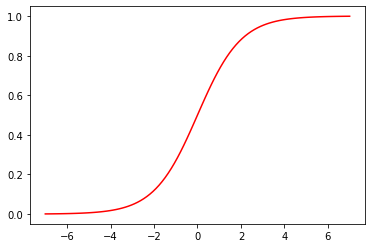
\includegraphics[width=0.6\textwidth]{sigmoid.png}
    \end{figure}

    Este algoritmo utiliza tanto una manera de clasificar como un método de
    actualización de pesos distintos. Ahora para clasificar cada uno de los puntos,
    en vez de usar la función $h$ anterior usaremos la función
    \emph{sigmoide} $\sigma$ (correspondiente al gráfico de arriba).

    \begin{equation*}
        \sigma (\textbf{x}) = \frac{1}{1 + e^{-f(\textbf{x})}} \;\;\; f(x) = \textbf{w}^\textbf{T}\textbf{x}
    \end{equation*}

    Y según esta función, el etiquetado para cada punto será:

    \begin{equation*}
        h(\textbf{x}) =
        \begin{cases}
            +1 & \sigma (\textbf{x}) \geq 0.5 \\
            -1 & \sigma (\textbf{x}) < 0.5 \\
        \end{cases}
    \end{equation*}

    De manera que ahora la clasificación de cada punto ahora depende de una probabilidad
    (el dominio de $\sigma$ es $[0,1]$ al igual que $\mathcal{P}$).
    La función $h$ ahora es una versión binaria de $\sigma$.

    ¿Y el error? Utilizaremos el \emph{cross-enthropy error}

    \begin{equation*}
        E_{in}(\textbf{w}) = \frac{1}{N}\sum^{N}_{n=1}{\ln\bigl(1 + e^{-y_n\textbf{w}^\textbf{T}\textbf{x}_n}\bigr)}
    \end{equation*}

    \paragraph*{Nota}$N = |\mathcal{D}|$

    \pagebreak

    \subsubsection{Descripción del algoritmo y pseudocódigo}

    \begin{figure*}[h]
        \textbf{Pseudocódigo}
        \begin{algorithmic}
            \Function{SGDLR}{$\mathcal{D}$, $\mathcal{Y}$, $\eta$, $T$, $N$} \Comment{$N$ es el tamaño del \emph{batch}}
            \State{$\textbf{w} \gets 0_{d}$} \Comment{Vector de $d$ ceros. $d$ es la dimensión de $\mathcal{D}$.}
            \State{$\textbf{w}_{old} \gets \infty$} \Comment{Pesos de la época anterior.}
            \State{$t \gets 0$}
            
            \While{$t \leq T$ \textbf{and} $|| \textbf{w}_{old} - \textbf{w} || \geq 0.01$}
                \State{$t \gets t + 1$}
                \State{$M \gets elegir([1,|\mathcal{D}|],N)$} \Comment{$N$ números en $[1,|\mathcal{D}|]$ sin repeticiones}
                \State{$\nabla E_{in} = -\frac{1}{|M|}\sum^{M}_{n}{\frac{y_n\textbf{x}_n}{1 + e^{y_n \textbf{w}^\textbf{T}\textbf{x}_n}}}$}
                \State{$\textbf{w}_{old} \gets \textbf{w}$}
                \State{$\textbf{w} \gets \textbf{w} - \eta \nabla E_{in}$}
            \EndWhile

            \State{\Return{$(w, t)$}}
            \EndFunction
        \end{algorithmic}
    \end{figure*}

    Ahora el algoritmo irá iterando por épocas.
    Una época $t$ es una hipótesis $h$ identificada por sus pesos, es decir, estamos
    hablando de la clasificación de los puntos adoptada por $h$ con los pesos de esa época.
    Comenzaremos a partir del vector de pesos cero, en vez de un vector pasado como parámetro,
    y entraremos en un bucle en el que \textbf{w siempre} recibe una actualización.
    
    Entonces, ¿cuál es la condición de parada? $||\textbf{w}_{old} - \textbf{w} || < 0.01$

    Esto significa que si la actualización de los pesos no ha sido lo suficientemente
    significante, entonces podemos parar.
    Los pesos se actualizan mediante el gradiente del error dentro de la muestra ($\nabla E_{in}$)
    multiplicado por una tasa de aprendizaje $\eta$, un método muy similar al de la práctica anterior.
    Estamos \textbf{minimizando} $E_{in}$, entonces es fácil caer en que $\nabla E_{in}$ es la derivada
    de $E_{in}$ \emph{cross-enthropy}.
    \linebreak

    ¿Por qué escogemos puntos aleatorios en cada época? Con esto podemos asegurar que
    los pesos que estamos intentando obtener sean más tolerables al resto de puntos y que no
    solo se centren en una elección para evitar errores en ciertos casos particulares.

    A continuación vamos a realizar ejecuciones de nuestro algoritmo, pero no tenemos una $\eta$
    y $N$ predeterminadas, por tanto tendremos que realizar varias ejecuciones experimentales para 
    decidirlo.

    \pagebreak

    \subsubsection{Escogiendo los parámetros}

    Vamos a ejecutar el algoritmo en un nuevo subconjunto de datos $\mathcal{D}$ donde $\mathcal{X} = [0,2] \times [0,2]$

    Para todas las ejecuciones ajustaremos $T = 1000$.

    Vamos a probar primero con $\eta = 0.1$ (igual que la práctica anterior)
    y $N = 80$ (igual que el \% de training). Se irán registrando los datos en la tabla
    si se nota un cambio en el porcentaje de aciertos o en el número de épocas $t$.

    \begin{figure*}[h]
        \centering
        \begin{tabular}{ |c|c|c|c|c|c| }
            \hline
            $\eta$ & $N$ & \textbf{w} & $E_{in}$ & Acierto(\%) & $t$ \\
            \hline
            $0.1$ & $80$ & $[-0.447, -0.477, 2.574]$ & $0.525$ & $82$ & $79$ \\
            \hline
            $0.25$ & $80$ & $[-1.287, -0.8, 1.989]$ & $0.425$ & $86$ & $118$ \\
            \hline
            $0.5$ & $80$ & $[-1.973, -0.787, 2.574]$ & $0.395$ & $87$ & $118$ \\
            \hline
            $0.7$ & $80$ & $[-2.284, -0.742, 2.78]$ & $0.387$ & $88$ & $112$ \\
            \hline
            $1.4$ & $80$ & $[-2.714, -0.632, 3.067]$ & $0.38$ & $89$ & $87$ \\
            \hline
            $1.6$ & $80$ & $[-3.404, -0.58, 3.5]$ & $0.376$ & $91$ & $223$ \\
            \hline
        \end{tabular}
    \end{figure*}

    Paro el experimento porque se ha alcanzado una tasa de acierto superior al 90\%
    A continuación mostraré una gráfica por ejecución de la tabla, ordenadas como en la tabla, 
    para que se vea el ajuste de $\eta$. Además, con $N$ no creo que haya problema ya que sigue
    la filosofía de la separación de los datos de entrenamiento y test.

    En conclusión, usaremos $\eta = 1.6$ y $N = 80$.

    \paragraph*{¿Cómo imprimimos la frontera de clasificación generada?}
    Hay que realizar un razonamiento matemático.

    \begin{equation*}
        \frac{1}{1 + e^{-f(x)}} = 0.5
    \end{equation*}
    \begin{equation*}
        \frac{1}{2} + \frac{e^{-f(x)}}{2} = 1
    \end{equation*}
    \begin{equation*}
        e^{-f(x)} = 1
    \end{equation*}
    \begin{equation*}
        f(x) = w_2x_2 + w_1x_1 + w_0 = 0
    \end{equation*}
    \begin{equation*}
        x_2 = \frac{-w_0 - w_1x_1}{w_2}
    \end{equation*}

    Para saber el porqué, véase la tercera línea de texto de la página 10, donde explica el
    significado de los componentes de \textbf{x}.

    \begin{figure}
        \centering
        $\eta = 0.1$
        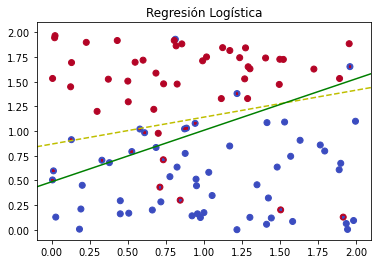
\includegraphics[width=0.6\textwidth]{rl1.png}
    \end{figure}

    \begin{figure}
        \centering
        $\eta = 0.25$
        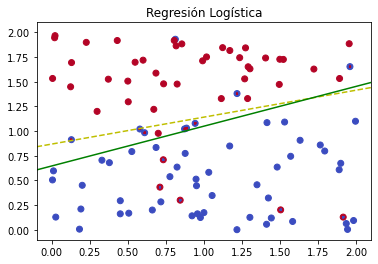
\includegraphics[width=0.6\textwidth]{rl2.png}
    \end{figure}

    \begin{figure}
        \centering
        $\eta = 0.5$
        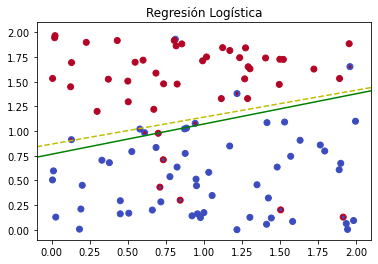
\includegraphics[width=0.6\textwidth]{rl3.png}
    \end{figure}

    \begin{figure}
        \centering
        $\eta = 0.7$
        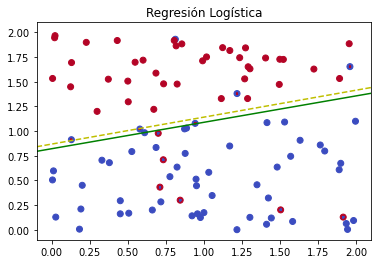
\includegraphics[width=0.6\textwidth]{rl4.png}
    \end{figure}

    \begin{figure}
        \centering
        $\eta = 1.4$
        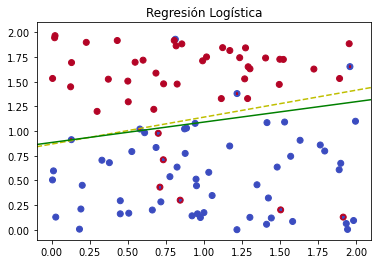
\includegraphics[width=0.6\textwidth]{rl5.png}
    \end{figure}

    \begin{figure}
        \centering
        $\eta = 1.6$
        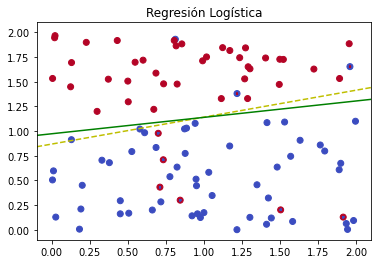
\includegraphics[width=0.6\textwidth]{rl6.png}
    \end{figure}

    \pagebreak
    \pagebreak

    \subsubsection{Experimentación con muestras grandes para el test}

    Emplearemos la última ejecución de nuestro algoritmo durante el experimento anterior
    para saber si clasifica bien en otros conjuntos de datos más grandes.

    Emplearemos $|\mathcal{D}_{test}| = 1200$ y repetiremos este experimento 100 veces.

    Si hacemos la media del error, el porcentaje de acierto y de epocas empleadas:

    \begin{figure*}[h]
        \centering
        \begin{tabular}{ |c|c|c| }
            \hline
            $E_{out}$ & Acierto(\%) & $t$ \\
            \hline
            0.408 & 0.881 & 353.58 \\
            \hline
        \end{tabular}
    \end{figure*}

    \begin{figure}[h]
        \centering
        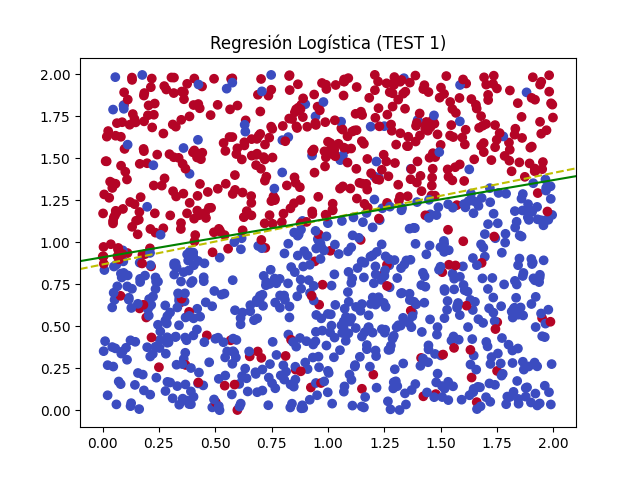
\includegraphics[width=0.6\textwidth]{rl7.png}
    \end{figure}

    Los resultados son buenos ya que $E_{in} \approx E_{out}$ y la tasa de acierto es $\approx 0.9$.

\end{document}